\begin{frame}[t]{Prueba de conexiones}\vspace{10pt}

Existen tres maneras de probar conexiones el\'ectricas - electr\'onicas:

\begin{enumerate}
	\item Pruebas de \textbf{continuidad}.
	\item A ciegas... funciona o no funciona. 
	\item Si no funciona: pruebas de diferencia de potencial - \textbf{voltaje} (Arduino maneja \textbf{5V}).
\end{enumerate}

\begin{figure}
	\centering
	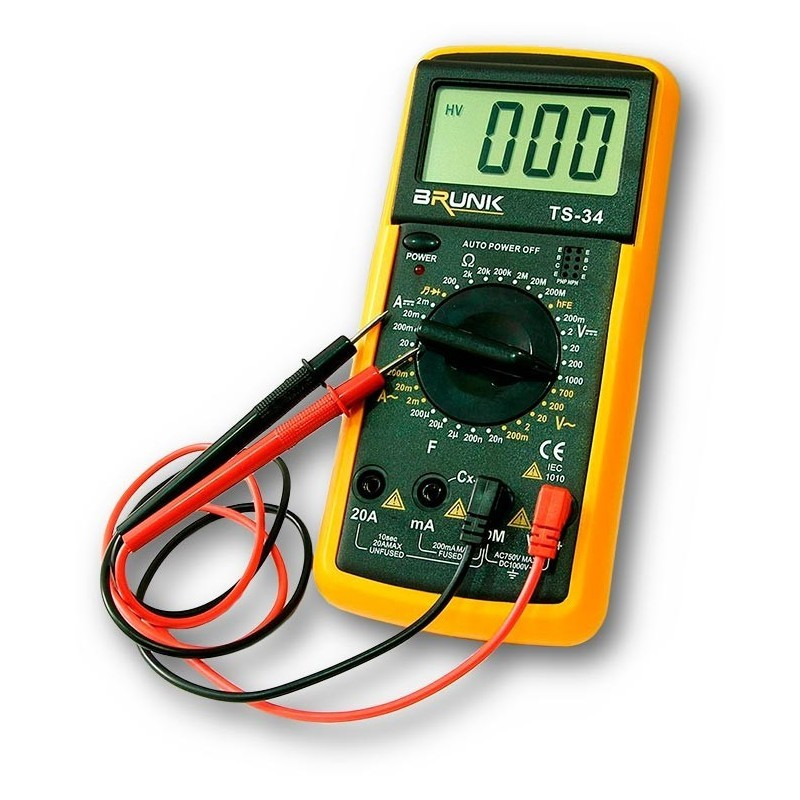
\includegraphics[scale=0.18]{Images/mult.jpg}
\end{figure}

\end{frame}